\chapter{Interactive Workload}

\section{Choke Points}

The design of the interactive workload queries has been conceived around two
main aspects: realism and technological relevance.  While realism has been
assessed by looking at existing social networks and thinking about what
interesting functionalities a user might desire from them, technological
relevance has been achieved by identifying a set of choke points queries should
stress.  These choke points capture those critical operations, techniques or
technologies that  could significatively affect the performance of the queries.
The choke points can be summarized in the following list:

% http://wiki.ldbcouncil.org/display/TUC/Interactive+Choke+Points

\subsection{Aggregation Performance}

The queries generally have a top-$k$ order by and often a group by in
addition to this.  These offer multiple optimization opportunities.
The queries also often have distinct operators, \ie distinct friends
within two steps.  Collectively these are all set operations that may
be implemented with some combination of hash and sorting, possibly
exploiting ordering in the data itself.  The aggregates are not
limited to counts and sums.  For example string concatenation occurs
as an aggregate, testing possible user defined aggregate support.
There is a wide range of cardinalities in grouping, from low, \eg country, to high, \eg post.

\subsection{Join Performance}

Each graph traversal step is in principle a join.  The join patterns are
diverse, exercising both index- and hash-based operators.   Queries are designed
so as to reward judicious use of hash join by having patterns starting with one
entity, fetching many related entities and then testing how these are related
to a third entity, \eg posts of a user with a tag of a given type.

\subsection{Data Access Locality}

Graph problems are notoriously non-local.  However, when queries touch
any non-trivial fraction of a dataset, locality will emerge and can be
exploited, for example by vectored index access or by ordering data so
that that a merge join is possible.

\subsection{Expression Calculation}

Queries often have expressions, including conditional expressions.
This provides opportunities for vectoring and tests efficient
management of intermediate results.

\subsection{Correlated Subqueries}

The workload has many correlated subqueries, for example constructts
like x within two steps but not in one step, which would typically be
a correlated subquery with NOT EXISTS.  There are also scalar
subqueries with aggregation, for example returning the count of posts
satisfying a certain criteria.


\subsection{Parallelism and Concurrency}

All queries offer opportunities for parallelism.  This tests a wide
range of constructs, for example partitioned parallel variants of
group by and distinct.  An interactive workload will typically avoid
trivially parallelizable table scans.  Thus the opportunities that
exist must be captured by index based, navigational query plans.  The
choice of whether to parallelize or not is often left to run time and
will have to depend on the actual data seen in the execution, as
starting a parallel thread with too little to do is
counter-productive.


\subsection{Graph Specifics}

Graph problems are generally characterized by transitive properties
and the fact that neighboring vertices often have a large overlap in
their environments.  This makes cardinality estimation harder.  For
example, a query optimizer needs to recognize whether a relationship
has a tree or graph shape in order to make correct cardinality
estimations.  Further, there are problems aggregating properties over
a set of consecutive edges.  The workload contains business questions
dealing with paths and aggregates across paths, as well as the easier
case of determining a membership in a hierarchy with a transitive
part-of relation.


\section{Query Specifications}

\subsection{Complex Reads Query Descriptions}
\label{sub:queries}

Notes:
\begin{itemize}
    \item Some queries require returning the content of a post. As stated in the
        schema, posts have either some content or an imageFile, but not both. An empty string in
        content represents the post not having any content, therefore, it must have a
        non-empty string in imageFile or the other way around.
\end{itemize}

{\small
    \begin{enumerate}
        \item Friends with certain name
            \begin{itemize}
                \item \textbf{Description:}
                    Given a start Person, find Persons with a given first name
                    that the start Person is connected to (excluding start Person) by
                    at most 3 steps via Knows relationships. Return Persons, including
                    summaries of the Persons workplaces and places of study.
                \item \textbf{Parameters:} \\
                    \begin{tabular}{ll}
                        Person.id 										& ID \\
                        Person.firstName								& String \\
                    \end{tabular}
                \item \textbf{Results:} \\
                    \begin{tabular}{ll}
                        Person.id 										& ID \\
                        Person.lastName									& String \\
                        Person.birthday 								& Date \\
                        Person.creationDate 							& DateTime  \\
                        Person.gender 									& String \\
                        Person.browserUsed 								& String \\
                        Person.locationIP 								& String \\
                        \{Person.emails\} 								& \{String\} \\
                        \{Person.language\}  							& \{String\} \\
                        Person-isLocatedIn->Place.name 				& String \\
                        \{Person-studyAt->University.name, \\
                            Person-studyAt->.classYear,  \\
                        Person-studyAt->University-isLocatedIn->City.name\}	& \{<String, 32-bit Integer, String>\} \\
                            \{Person-workAt->Company.name, \\
                                Person-workAt->.workFrom, \\
                            Person-workAt->Company-isLocatedIn->Country.name\} & \{<String, 32-bit Integer, String>\} \\
                            \end{tabular}
                \item \textbf{Sort:}
                            \begin{itemize}
                              \item[1st] distance from person (ascending)
                              \item[2nd] Person.lastName (ascending)
                              \item[3rd] Person.id (ascending)
                            \end{itemize}
                \item \textbf{Limit:}
                  \begin{itemize}
                    \item[] 20
                  \end{itemize}
              \end{itemize}

                \item Recent posts and comments by your friends
                    \begin{itemize}
                        \item \textbf{Description:}
                          Given a start Person, find (most recent) Messages from
                            all of that Person's friends, that were created before (and
                            including) a given date.
                        \item \textbf{Parameters:} \\
                            \begin{tabular}{ll}
                                Person.id 										& ID \\
                                date 											& DateTime \\
                            \end{tabular}
                        \item \textbf{Results:} \\
                            \begin{tabular}{ll}
                              Message-hasCreator->Person.id 										& ID \\
                                ssage-hasCreator->Person.firstName								& String \\
                                ssage-hasCreator->Person.lastName									& String \\
                                Message.id 								& ID \\
                                Message.content or Post.imageFile 	& String \\
                                Message.creationDate	& DateTime \\
                            \end{tabular}
                        \item \textbf{Sort:}
                          \begin{itemize}
                            \item[1st] Message.creationDate (descending)
                            \item[2nd] Message.id (ascending)
                          \end{itemize}
                \item \textbf{Limit:}
                  \begin{itemize}
                    \item[] 20
                  \end{itemize}
                    \end{itemize}

                \item Friends and friends of friends that have been to countries X and Y
                    \begin{itemize}
                        \item \textbf{Description:}
                            Given a start Person, find Persons that are their friends and
                            friends of friends (excluding start Person) that have made
                            Posts/Comments in both of the given Countries, X and Y, within a
                            given period.  Only Persons that are foreign to Countries X and Y
                            are considered, that is Persons whose Location is not Country X or
                            Country Y.
                        \item \textbf{Parameters:} \\
                            \begin{tabular}{lll}
                                Person.id 										& ID & \\
                                CountryX.name									& String & \\
                                CountryY.name									& String & \\
                                startDate										& Date 	& // beginning of requested period \\
                                duration										& 32-bit Integer 					& // duration of requested period, in days \\
                                                  &                                   & // the interval [startDate, startDate + Duration) is closed-open\\
                            \end{tabular}
                        \item \textbf{Results:} \\
                            \begin{tabular}{lll}
                                Person.id 										& ID 	& \\
                                Person.firstName 								& String 			& \\
                                Person.lastName 								& String 			& \\
                                countx 											& 32-bit Integer 	&
                                \parbox[t]{20cm}{// number of Messages from Country X made by Person \par
                            within the given time\strut} \\
                            county 											& 32-bit Integer 	&
                            \parbox[t]{20cm}{// number of Messages from Country Y made by Person \par
                        within the given time\strut} \\
                        count 											& 32-bit Integer 	& // countx + county \\
                    \end{tabular}
                        \item \textbf{Sort:}
                          \begin{itemize}
                            \item[1st] countx (descending)
                            \item[2nd] Person.id (ascending)
                          \end{itemize}
                        \item \textbf{Limit:}
                          \begin{itemize}
                            \item[] 20
                          \end{itemize}
            \end{itemize}

        \item New topics
            \begin{itemize}
                \item \textbf{Description:}
                    Given a start Person, find Tags that are attached to Posts that
                    were created by that Person's friends.  Only include Tags that were
                    attached to friends' Posts created within a given time interval, and that
                    were never attached to friends' Posts created before this interval.
                \item \textbf{Parameters:} \\
                    \begin{tabular}{lll}
                        Person.id 										& ID 	& \\
                        startDate 										& Date & \\
                        duration										& 32-bit Integer 					& // duration of requested period, in days \\
                                          &                                   & // the interval [startDate, startDate + Duration) is closed-open\\
                    \end{tabular}
                \item \textbf{Results:} \\
                    \begin{tabular}{lll}
                        Tag.name 										& String 	& \\
                        count 											& 32-bit Integer & // number of Posts made within the given time interval that have this Tag \\
                    \end{tabular}
                \item \textbf{Sort:}
                  \begin{itemize}
                    \item[1st] count (descending)
                    \item[2nd] Tag.name (ascending)
                  \end{itemize}
                        \item \textbf{Limit:}
                          \begin{itemize}
                            \item[] 10
                          \end{itemize}
            \end{itemize}

        \item New groups
            \begin{itemize}
                \item \textbf{Description:}
                    Given a start Person, find the Forums which that Person's friends
                    and friends of friends (excluding start Person) became Members of
                    after a given date.  For each forum find the number of Posts
                    that were created by any of these Persons.
                    For each Forum and consider only
                    those Persons which joined that particular
                    Forum after the given date.
                \item \textbf{Parameters:} \\
                    \begin{tabular}{lll}
                        Person.id 										& ID & \\
                        date 											& Date & \\
                    \end{tabular}
                \item \textbf{Results:} \\
                    \begin{tabular}{lll}
                        Forum.title 										& String & \\
                        count 	 											& 32-bit Integer & \parbox[t]{20cm}{// number of Posts made in Forum that were created 																							by friends \par \strut} \\
                    \end{tabular}
                \item \textbf{Sort:}
                  \begin{itemize}
                    \item[1st] count (descending)
                    \item[2nd] Forum.id (ascending)
                  \end{itemize}
                \item \textbf{Limit:}
                  \begin{itemize}
                    \item[] 20
                  \end{itemize}
            \end{itemize}

        \item Tag co-occurrence
            \begin{itemize}
                \item \textbf{Description:}
                    Given a start Person and some Tag, find the other Tags that occur
                    together with this Tag on Posts that were created by start Person's
                    friends and friends of friends (excluding start Person).  Return
                    For each Tag, find the count of Posts that were created by these
                    Persons, which contain both this Tag and the given Tag.
                \item \textbf{Parameters:} \\
                    \begin{tabular}{lll}
                        Person.id 										& ID & \\
                        Tag.name 	 									& String & \parbox[t]{20cm}{\par \strut} \\
                    \end{tabular}
                \item \textbf{Results:} \\
                    \begin{tabular}{lll}
                        Tag.name 	 						& String & \parbox[t]{20cm}{\par \strut} \\
                        count 								& 32-bit Integer & \parbox[t]{20cm}{// number of Posts that were created by friends and friends of friends, \par
                    which contain this Tag\strut} \\
                \end{tabular}
                \item \textbf{Sort:}
                  \begin{itemize}
                    \item[1st] count (descending)
                    \item[2nd] Tag.name (ascending)
                  \end{itemize}
                \item \textbf{Limit:}
                  \begin{itemize}
                    \item[] 10
                  \end{itemize}
        \end{itemize}

      \item Recent likers
        \begin{itemize}
            \item \textbf{Description:}
                Given a start Person, find (most recent) Likes on any of start
                Person's Messages.  Find Persons that Liked any of start
                Person's Messages, the Messages they liked most recently,
                creation date of that Like, and the latency (in minutes) between
                creation of Messages and Like.  Additionally, for each Person
                found return a flag indicating whether the liker is a friend of
                start Person.  In the case that a Person Liked multiple Messages
                at the same time, return the Message with lowest identifier.
            \item \textbf{Parameters:} \\
                \begin{tabular}{lll}
                    Person.id 	 						& 64-bit Integer & \parbox[t]{20cm}{\par \strut} \\
                \end{tabular}
            \item \textbf{Results:} \\
                \begin{tabular}{lll}
                    Person.id 	 								& ID & \parbox[t]{20cm}{\par \strut} \\
                    Person.firstName 							& String & \parbox[t]{20cm}{\par \strut} \\
                    Person.lastName 	 						& String & \parbox[t]{20cm}{\par \strut} \\
                    Like.creationDate 	 						& DateTime & \parbox[t]{20cm}{\par \strut} \\
                    Message.id 	 						& ID & \parbox[t]{20cm}{\par \strut} \\
                    Message.content or Post.imageFile	& String & \parbox[t]{20cm}{\par \strut} \\
                    latency 	 								& 32-bit Integer &
                    \parbox[t]{20cm}{// duration between creation of\par Message and Like, in minutes\strut} \\
                    isNew										& Boolean & \parbox[t]{20cm}{// false if liker Person is friend of\par start Person, true otherwise \strut} \\
                \end{tabular}
             \item \textbf{Sort:}
                  \begin{itemize}
                    \item[1st] Like.creationDate (descending)
                    \item[2nd] Person.id (ascending)
                  \end{itemize}
                \item \textbf{Limit:}
                  \begin{itemize}
                    \item[] 20
                  \end{itemize}
        \end{itemize}

    \item Recent replies
        \begin{itemize}
            \item \textbf{Description:}
                Given a start Person, find (most recent) Comments that are replies
                to Messages of the start Person. Only consider immediate
                (1-hop) replies, not the transitive (multi-hop) case.  Return the
                reply Comments, and the Person that created each reply
                Comment.
            \item \textbf{Parameters:} \\
                \begin{tabular}{lll}
                    Person.id 	 						& ID & \parbox[t]{20cm}{\par \strut} \\
                \end{tabular}
            \item \textbf{Results:} \\
                \begin{tabular}{lll}
                    Person.id 	 				& ID & \parbox[t]{20cm}{\par \strut} \\
                    Person.firstName 	 		& String & \parbox[t]{20cm}{\par \strut} \\
                    Person.lastName 	 		& String & \parbox[t]{20cm}{\par \strut} \\
                    Comment.creationDate 	 	& DateTime & \parbox[t]{20cm}{\par \strut} \\
                    Comment.id 	 				& ID & \parbox[t]{20cm}{\par \strut} \\
                    Comment.content 	 		& String & \parbox[t]{20cm}{\par \strut} \\
                \end{tabular}
             \item \textbf{Sort:}
                  \begin{itemize}
                    \item[1st] Comment.creationDate (descending)
                    \item[2nd] Comment.id (ascending)
                  \end{itemize}
              \item \textbf{Limit:}
                  \begin{itemize}
                    \item[] 20
                  \end{itemize}
        \end{itemize}

    \item Recent posts and comments by friends or friends of friends
        \begin{itemize}
            \item \textbf{Description:}
              Given a start Person, find the (most recent) Messages created
                by that Person's friends or friends of friends (excluding start
                Person). Only consider the Messages created before a given
                date (excluding that date).
            \item \textbf{Parameters:} \\
                \begin{tabular}{lll}
                    Person.id 	 						& ID & \parbox[t]{20cm}{\par \strut} \\
                    date 		 						& Date & \parbox[t]{20cm}{\par \strut} \\
                \end{tabular}
            \item \textbf{Results:} \\
                \begin{tabular}{lll}
                  Message-hasCreator->Person.id 	 								& ID & \parbox[t]{20cm}{\par \strut} \\
                  Message-hasCreator->Person.firstName 	 						& String & \parbox[t]{20cm}{\par \strut} \\
                  Message-hasCreatr->Person.lastName 	 						& String & \parbox[t]{20cm}{\par \strut} \\
                    Message.id  	 						& ID & \parbox[t]{20cm}{\par \strut} \\
                    Message.content or Post.imageFile	& String & \parbox[t]{20cm}{\par \strut} \\
                    Message.creationDate 	 	& DateTime & \parbox[t]{20cm}{\par \strut} \\
                \end{tabular}
             \item \textbf{Sort:}
                  \begin{itemize}
                    \item[1st] Message.creationDate (descending)
                    \item[2nd] Message.id (ascending)
                  \end{itemize}
             \item \textbf{Limit:}
                  \begin{itemize}
                    \item[] 20
                  \end{itemize}
        \end{itemize}

    \item Friend recommendation
        \begin{itemize}
            \item \textbf{Description:}
                Given a start Person, find that Person's friends of friends
                (excluding start Person, and immediate friends), who were born on
                or after the 21st of a given month (in any year) and before the
                22nd of the following month.  Calculate the similarity between each
                of these Persons and start Person, where similarity for any Person
                is defined as follows:
                \begin{itemize}
                    \item common = number of Posts created by that Person, such that the Post has a Tag that start Person is Interested in
                    \item uncommon = number of Posts created by that Person, such that the Post has no Tag that start Person is Interested in
                    \item similarity = common - uncommon
                \end{itemize}
            \item \textbf{Parameters:} \\
                \begin{tabular}{lll}
                    Person.id 	 						& ID & \parbox[t]{20cm}{\par \strut} \\
                    month 		 						& 32-bit Integer & \parbox[t]{20cm}{// between 1-12\par \strut} \\
                \end{tabular}
            \item \textbf{Results:} \\
                \begin{tabular}{lll}
                    Person.id 	 						& ID & \parbox[t]{20cm}{\par \strut} \\
                    Person.firstName 	 				& String & \parbox[t]{20cm}{\par \strut} \\
                    Person.lastName 	 				& String & \parbox[t]{20cm}{\par \strut} \\
                    similarity 	 						& 32-bit Integer & \parbox[t]{20cm}{\par \strut} \\
                    Person.gender 	 					& String & \parbox[t]{20cm}{\par \strut} \\
                    Person-isLocatedIn->Place.name 	    & Sting & \parbox[t]{20cm}{\par \strut} \\
                \end{tabular}
            \item \textbf{Sort:}
                  \begin{itemize}
                    \item[1st] similarity (descending)
                    \item[2nd] Person.id (ascending)
                  \end{itemize}
             \item \textbf{Limit:}
                  \begin{itemize}
                    \item[] 10
                  \end{itemize}
        \end{itemize}

    \item Job referral
        \begin{itemize}
            \item \textbf{Description:}
                Given a start Person, find that Person's friends and friends of
                friends (excluding start Person) who started Working in some
                Company in a given Country, before a given date (year).
            \item \textbf{Parameters:} \\
                \begin{tabular}{lll}
                    Person.id 	 				& ID & \parbox[t]{20cm}{\par \strut} \\
                    Country.name 	 			& String & \parbox[t]{20cm}{\par \strut} \\
                    year 		 				& 32-bit Integer & \parbox[t]{20cm}{\par \strut} \\
                \end{tabular}
            \item \textbf{Results:} \\
                \begin{tabular}{lll}
                    Person.id 	 						& ID & \parbox[t]{20cm}{\par \strut} \\
                    Person.firstName 	 				& String & \parbox[t]{20cm}{\par \strut} \\
                    Person.lastName 	 				& String & \parbox[t]{20cm}{\par \strut} \\
                    Person-worksAt->Organization.name 	& String & \parbox[t]{20cm}{\par \strut} \\
                    Person-worksAt->.worksFrom 	 		& 32-bit Integer & \parbox[t]{20cm}{\par \strut} \\
                \end{tabular}
            \item \textbf{Sort:}
                  \begin{itemize}
                    \item[1st] Person-worksAt->.worksFrom (ascending)
                    \item[2nd] Person.id (ascending)
                    \item[3st] Person-worksAt->Organization.name (descending)
                  \end{itemize}
            \item \textbf{Limit:}
                  \begin{itemize}
                    \item[] 10
                  \end{itemize}
        \end{itemize}

    \item Expert search
        \begin{itemize}
            \item \textbf{Description:}
                Given a start Person, find the Comments that this Person's
                friends made in reply to Posts, considering only those Comments
                that are immediate (1-hop) replies to Posts, not the transitive
                (multi-hop) case.  Only consider Posts with a Tag in a given
                TagClass or in a descendent of that TagClass.  Count the number
                of these reply Comments, and collect the Tags (with valid tag
                class) that were attached to the Posts they replied to.  Return
                Persons with at least one reply, the reply count, and
                the collection of Tags.
            \item \textbf{Parameters:} \\
                \begin{tabular}{lll}
                    Person.id 	 					& ID & \parbox[t]{20cm}{\par \strut} \\
                    TagClass.name	 				& String & \parbox[t]{20cm}{\par \strut} \\
                \end{tabular}
            \item \textbf{Results:} \\
                \begin{tabular}{lll}
                    Person.id 	 			& ID & \parbox[t]{20cm}{\par \strut} \\
                    Person.firstName 	 	& String & \parbox[t]{20cm}{\par \strut} \\
                    Person.lastName 	 	& String & \parbox[t]{20cm}{\par \strut} \\
                    \{Tag.name\} 	 			& \{String\} & \parbox[t]{20cm}{\par \strut} \\
                    count 	 				& 32-bit Integer & \parbox[t]{20cm}{// number of reply Comments\par \strut}
                \end{tabular}
            \item \textbf{Sort:}
                  \begin{itemize}
                    \item[1st] count (descending)
                    \item[2nd] Person.id (ascending)
                  \end{itemize}
            \item \textbf{Limit:}
                  \begin{itemize}
                    \item[] 20
                  \end{itemize}
        \end{itemize}

    \item Single shortest path
        \begin{itemize}
            \item \textbf{Description:}
                Given two Persons, find the shortest path between these two Persons in the subgraph induced by the Knows relationships.
                Return the length of this path.
                \begin{itemize}
                    \item -1 : no path found
                    \item 0: start person = end person
                    \item > 0: regular case
                \end{itemize}
            \item \textbf{Parameters:} \\
                \begin{tabular}{lll}
                    Person.id 	 			& ID & \parbox[t]{20cm}{// person 1\strut} \\
                    Person.id 	 			& ID & \parbox[t]{20cm}{// person 2\strut} \\
                \end{tabular}
            \item \textbf{Results:} \\
                \begin{tabular}{lll}
                    length 	 			& 32-bit Integer & \parbox[t]{20cm}{\par \strut} \\
                \end{tabular}
            \item \textbf{Sort:}
                  \begin{itemize}
                    \item[] -
                  \end{itemize}
            \item \textbf{Limit:}
                  \begin{itemize}
                    \item[] -
                  \end{itemize}
        \end{itemize}

    \item Weighted/unweighted paths
        \begin{itemize}
            \item \textbf{Description:}
                Given two Persons, find all (unweighted) shortest paths between
                these two Persons, in the subgraph induced by the Knows
                relationship. Then, for each path calculate a weight.  The nodes in
                the path are Persons, and the weight of a path is the sum of
                weights between every pair of consecutive Person nodes in the path.
                The weight for a pair of Persons is calculated such that every
                reply (by one of the Persons) to a Post (by the other Person)
                contributes 1.0, and every reply (by ones of the Persons) to a
                Comment (by the other Person) contributes 0.5. Return all the
                paths with shortest length, and their weights.
            \item \textbf{Parameters:} \\
                \begin{tabular}{lll}
                    Person.id 	 			& ID & \parbox[t]{20cm}{// person 1\strut} \\
                    Person.id 	 			& ID & \parbox[t]{20cm}{// person 2\strut} \\
                \end{tabular}
            \item \textbf{Results:} \\
                \begin{tabular}{lll}
                    [Person.id] 	& [ID] & \parbox[t]{20cm}{// Identifiers representing an ordered sequence of the Persons in the path \strut} \\
                    weight 	 					& 64-bit Float & \parbox[t]{20cm}{\strut} \\
                \end{tabular}
            \item \textbf{Sort:}
                  \begin{itemize}
                    \item[1st] weight (descending) // The order of paths with
                      the same weight is unspecified
                  \end{itemize}
            \item \textbf{Limit:}
                  \begin{itemize}
                    \item[] -
                  \end{itemize}
        \end{itemize}
\end{enumerate}
}

\subsection{Short Reads Query Descriptions}

{\small
\begin{enumerate}

  \item Person Profile
    \begin{itemize}
      \item \textbf{Description:}
        Given a start Person, retrieve their first name, last name, birthday, IP address, browser, and city of residence.
      \item \textbf{Parameters:} \\
        \begin{tabular}{lll}
          Person.id 										& ID \\
        \end{tabular}
      \item \textbf{Results:} \\
        \begin{tabular}{lll}
          Person.firstName									& String \\
          Person.lastName										& String \\
          Person.birthDay										& Date \\
          Person.locationIP									& String \\
          Person.browserUsed								& String \\
          Person-isLocatedIn->Place.id			& 32-bit Integer \\
          Person.gender									    & String \\
          Person.creationDate						    & DateTime \\
        \end{tabular}
            \item \textbf{Sort:}
                  \begin{itemize}
                    \item[] -
                  \end{itemize}
            \item \textbf{Limit:}
                  \begin{itemize}
                    \item[] -
                  \end{itemize}
    \end{itemize}

  \item Person Recent Messages
    \begin{itemize}
      \item \textbf{Description:}
        Given a start Person, retrieve the last 10 Messages created by that user.
        For each message, return that message, the original post in its conversation, and the author of that post.
        If any of the Messages is a Post, then the original Post will be the same Message, \ie that Message will appear twice in that result.
      \item \textbf{Parameters:} \\
        \begin{tabular}{lll}
          Person.id 										& ID \\
        \end{tabular}
      \item \textbf{Results:} \\
        \begin{tabular}{lll}
          Message.id     									& 64-bit Integer \\
          Message.content or Post.imageFile										& String \\
          Message.creationDate  & DateTime \\
          Post.id or Comment-replyOf*->Post.id								& ID \\
          Post-hasCreator->Person.id or Comment-replyOf*->Post-hasCreator->Person.id & ID \\
          Post-hasCreator->Person.firstName or Comment-replyOf*->Post-hasCreator->Person.firstName & String \\
          Post-hasCreator->Person.lastName or Comment-replyOf*->Post-hasCreator->Person.lastName & String \\
        \end{tabular}
      \item \textbf{Sort:}
        \begin{itemize}
          \item[1st] Message.creationDate (descending)
          \item[2nd] Message.id (descending)
        \end{itemize}
            \item \textbf{Limit:}
                  \begin{itemize}
                    \item[] -
                  \end{itemize}
    \end{itemize}

  \item Person Friends
    \begin{itemize}
      \item \textbf{Description:}
        Given a start Person, retrieve all of their friends, and the date at which they became friends.
      \item \textbf{Parameters:} \\
        \begin{tabular}{lll}
          Person.id 										& ID \\
        \end{tabular}
      \item \textbf{Results:} \\
        \begin{tabular}{lll}
          Person.id     									& ID \\
          Person.firstName     						& String \\
          Person.lastName    							& String \\
          Knows.creationDate    					& DateTime \\
        \end{tabular}
      \item \textbf{Sort:}
        \begin{itemize}
          \item[1st] Knows.creationDate (descending)
          \item[2nd] Person.id (ascending)
        \end{itemize}
            \item \textbf{Limit:}
                  \begin{itemize}
                    \item[] -
                  \end{itemize}
    \end{itemize}

  \item Message Content
    \begin{itemize}
      \item \textbf{Description:}
        Given a Message, retrieve its content and creation date.
      \item \textbf{Parameters:} \\
        \begin{tabular}{lll}
          Message.id 										& ID \\
        \end{tabular}
      \item \textbf{Results:} \\
        \begin{tabular}{lll}
          Message.creationDate   									& ID \\
          Message.content or Post.imageFile           										& String \\
        \end{tabular}
            \item \textbf{Sort:}
                  \begin{itemize}
                    \item[] -
                  \end{itemize}
            \item \textbf{Limit:}
                  \begin{itemize}
                    \item[] -
                  \end{itemize}
    \end{itemize}

  \item Message Creator
    \begin{itemize}
      \item \textbf{Description:}
        Given a Message, retrieve its author.
      \item \textbf{Parameters:} \\
        \begin{tabular}{lll}
          Message.id 										& ID \\
        \end{tabular}
      \item \textbf{Results:} \\
        \begin{tabular}{lll}
          Message-hasCreator->Person.id     									& ID \\
          Message-hasCreator->Person.firstName     									& String \\
          Message-hasCreator->Person.lastName    									& String \\
        \end{tabular}
            \item \textbf{Sort:}
                  \begin{itemize}
                    \item[] -
                  \end{itemize}
            \item \textbf{Limit:}
                  \begin{itemize}
                    \item[] -
                  \end{itemize}
    \end{itemize}

  \item Message Forum
    \begin{itemize}
      \item \textbf{Description:}
        Given a Message, retrieve the Forum that contains it
        and the Person that moderates that forum. Since comments are not
        directly contained in forums, for comments, return the forum containing
        the original post in the thread which the comment is replying to.
      \item \textbf{Parameters:} \\
        \begin{tabular}{lll}
          Message.id 										& ID \\
        \end{tabular}
      \item \textbf{Results:} \\
        \begin{tabular}{lll}
          Message<-containerOf-Forum.id                       & ID \\
          Message<-containerOf-Forum.title     									& String \\
          Message<-containerOf-Forum-hasModerator->Person.id     									& ID \\
          Message<-containerOf-Forum-hasModerator->Person.firstName    									& String \\
          Message<-containerOf-Forum-hasModerator->Person.lastName    									& String \\
        \end{tabular}
            \item \textbf{Sort:}
                  \begin{itemize}
                    \item[] -
                  \end{itemize}
            \item \textbf{Limit:}
                  \begin{itemize}
                    \item[] -
                  \end{itemize}
    \end{itemize}

  \item Message Replies
    \begin{itemize}
      \item \textbf{Description:}
        Given a Message, retrieve the (1-hop) Comments that reply to it.
        In addition, return a boolean flag indicating if the author of the reply knows the author of the original message.
        If author is same as original author, return false for "knows" flag.
      \item \textbf{Parameters:} \\
        \begin{tabular}{lll}
          Message.id 										& ID \\
        \end{tabular}
      \item \textbf{Results:} \\
        \begin{tabular}{lll}
          Message<-replyOf-Comment.id                       & ID \\
          Message<-replyOf-Comment.content                       & String \\
          Message<-replyOf-Comment.creationDate                       & DateTime \\
          Message-hasCreator->Person.id     									& ID \\
          Message-hasCreator->Person.firstName    									& String \\
          Message-hasCreator->Person.lastName     									& String \\
        \end{tabular}
      \item \textbf{Sort:}
        \begin{itemize}
          \item[1st] Message<-replyOf-Comment.creationDate (descending)
          \item[2nd] Message-hasCreator->Person.id (ascending)
        \end{itemize}
            \item \textbf{Limit:}
                  \begin{itemize}
                    \item[] -
                  \end{itemize}
    \end{itemize}
\end{enumerate}
}

\subsection{Update Query Descriptions}
{\small
\begin{enumerate}
    \item Add Person
        \begin{itemize}
            \item \textbf{Description:} Add a Person to the social network.
            \item \textbf{Parameters:} \\
                \begin{tabular}{lll}
                    Person.id 	 			& ID & \parbox[t]{20cm}{\par \strut} \\
                    Person.firstName 		& String & \parbox[t]{20cm}{\par \strut} \\
                    Person.lastName 		& String & \parbox[t]{20cm}{\par \strut} \\
                    Person.gender 		& String & \parbox[t]{20cm}{\par \strut} \\
                    Person.birthDay 		& Date & \parbox[t]{20cm}{\par \strut} \\
                    Person.creationDate     & DateTime & \parbox[t]{20cm}{\par \strut} \\
                    Person.locationIp     & String & \parbox[t]{20cm}{\par \strut} \\
                    Person.browserUsed     & String & \parbox[t]{20cm}{\par \strut} \\
                    Person-isLocatedIn->City.id 	& ID & \parbox[t]{20cm}{\par \strut} \\
                    Person.speaks 	& \{ String \} & \parbox[t]{20cm}{\par \strut} \\
                    Person.emails 	& \{ String \} & \parbox[t]{20cm}{\par \strut} \\
                    Person-hasInterest->Tag.id 	& \{ ID \} & \parbox[t]{20cm}{\par \strut} \\
                    \{ Person-studyAt->University.id, \\
                    Person-studyAt->.classYear \}  & \{ID, 32-bit Integer\} & \parbox[t]{20cm}{\par \strut} \\
                        \{ Person-workAt->Company.id, \\
                        Person-workAt->.workFrom \}  & \{ID, 32-bit Integer\} & \parbox[t]{20cm}{\par \strut} \\
                        \end{tabular}
                \end{itemize}
            \item Add Post Like
                \begin{itemize}
                    \item \textbf{Description:} Add a Like to a Post of the social network.
                    \item \textbf{Parameters:} \\
                        \begin{tabular}{lll}
                            Person.id 	 			& ID & \parbox[t]{20cm}{\par \strut} \\
                            Post.id 	 			& ID & \parbox[t]{20cm}{\par \strut} \\
                            Person-likes->.creationDate 	 		& DateTime & \parbox[t]{20cm}{\par \strut} \\
                        \end{tabular}
                \end{itemize}
            \item Add Comment Like
                \begin{itemize}
                    \item \textbf{Description: Add a Like to a Comment of the social network.}
                    \item \textbf{Parameters:} \\
                        \begin{tabular}{lll}
                            Person.id 	 			& ID & \parbox[t]{20cm}{\par \strut} \\
                            Comment.id 	 			& ID & \parbox[t]{20cm}{\par \strut} \\
                            Person-likes->.creationDate 	 		& DateTime & \parbox[t]{20cm}{\par \strut} \\
                        \end{tabular}
                \end{itemize}
            \item Add Forum
                \begin{itemize}
                    \item \textbf{Description:} Add a Forum to the social network.
                    \item \textbf{Parameters:} \\
                        \begin{tabular}{lll}
                            Forum.id 	 			& ID & \parbox[t]{20cm}{// person 1\strut} \\
                            Forum.title 	 			& String & \parbox[t]{20cm}{// person 2\strut} \\
                            Forum.creationDate & DateTime & \parbox[t]{20cm}{\par \strut} \\
                            Forum-hasModerator->Person.id 	& \{ ID \} & \parbox[t]{20cm}{\par \strut} \\
                            Forum-hasTag->Tag.id 	& \{ ID \} & \parbox[t]{20cm}{\par \strut} \\
                        \end{tabular}
                \end{itemize}
            \item Add Forum Membership
                \begin{itemize}
                    \item \textbf{Description:} Add a Forum membership to the social network.
                    \item \textbf{Parameters:} \\
                        \begin{tabular}{lll}
                            Person.id 	 			& ID & \parbox[t]{20cm}{\par \strut} \\
                            Person-hasMember->Forum.id 	 			& ID & \parbox[t]{20cm}{\par \strut} \\
                            Person-hasMember->.joinDate 	 		& DateTime & \parbox[t]{20cm}{\par \strut} \\
                        \end{tabular}
                \end{itemize}
            \item Add Post
                \begin{itemize}
                    \item \textbf{Description:} Add a Post to the social network.
                    \item \textbf{Parameters:} \\
                        \begin{tabular}{lll}
                            Post.id 	 			& ID & \parbox[t]{20cm}{\par \strut} \\
                            Post.imageFile 	 			& String & \parbox[t]{20cm}{\par \strut} \\
                            Post.creationDate 	 		& DateTime & \parbox[t]{20cm}{\par \strut} \\
                            Post.locationIp 	 		& String & \parbox[t]{20cm}{\par \strut} \\
                            Post.browserUsed 	 		& String & \parbox[t]{20cm}{\par \strut} \\
                            Post.language 	 		    & String & \parbox[t]{20cm}{\par \strut} \\
                            Post.content 	 		    & Text & \parbox[t]{20cm}{\par \strut} \\
                            Post.length 	 		    & 32-bit Integer & \parbox[t]{20cm}{\par \strut} \\
                            Post-hasCreator->Person.id & ID & \parbox[t]{20cm}{\par \strut} \\
                            Forum-containerOf->Post.id & ID & \parbox[t]{20cm}{\par \strut} \\
                            Post-isLocatedIn->Country.id & ID & \parbox[t]{20cm}{\par \strut} \\
                            \{Post-hasTag->Tag.id\} & \{ID\} & \parbox[t]{20cm}{\par \strut} \\
                        \end{tabular}
                \end{itemize}
            \item Add Comment
                \begin{itemize}
                    \item \textbf{Description:} Add a Comment replying to a Post/Comment to the social network.
                    \item \textbf{Parameters:} \\
                        \begin{tabular}{lll}
                            Comment.id 	 			& ID & \parbox[t]{20cm}{\par \strut} \\
                            Comment.creationDate 			& DateTime & \parbox[t]{20cm}{\par \strut} \\
                            Comment.locationIp 	 		& String & \parbox[t]{20cm}{\par \strut} \\
                            Comment.browserUsed 	 		& String & \parbox[t]{20cm}{\par \strut} \\
                            Comment.content 	 		    & Text & \parbox[t]{20cm}{\par \strut} \\
                            Comment.length 	 		    & 32-bit Integer & \parbox[t]{20cm}{\par \strut} \\
                            Comment-hasCreator->Person.id & ID & \parbox[t]{20cm}{\par \strut} \\
                            Comment-isLocatedIn->Country.id & ID & \parbox[t]{20cm}{\par \strut} \\
                            Comment-replyOf->Post.id & ID & \parbox[t]{20cm}{ // -1 if the comment is a reply of a comment. \strut} \\
                            Comment-replyOf->Comment.id & ID & \parbox[t]{20cm}{// -1 if the comment is a reply of a post. \strut} \\
                            \{Comment-hasTag->Tag.id\} & \{ID\} & \parbox[t]{20cm}{\par \strut} \\
                        \end{tabular}
                \end{itemize}
            \item Add Friendship
                \begin{itemize}
                    \item \textbf{Description:} Add a friendship relation to the social network
                    \item \textbf{Parameters:} \\
                        \begin{tabular}{lll}
                            Person.id 	 			& ID & \parbox[t]{20cm}{// person 1\strut} \\
                            Person.id 	 			& ID & \parbox[t]{20cm}{// person 2\strut} \\
                            Person-knows->.creationDate & DateTime & \parbox[t]{20cm}{\par \strut} \\
                        \end{tabular}
                \end{itemize}
        \end{enumerate}
      }

\renewcommand*{\arraystretch}{1.1}

\noindent\begin{tabularx}{17cm}{|p{1.95cm}|X|}
	\hline
	number      & 1                                                          \\ \hline
%
	title       & Friends with certain name                                                           \\ \hline
	\multicolumn{2}{|c|}{ 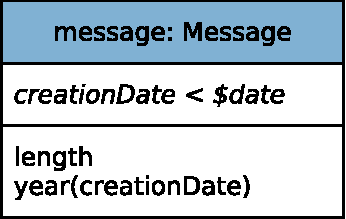
\includegraphics[scale=\patternscale,margin=0cm .2cm]{patterns/q01}} \\ \hline
	description & Given a start Person, find Persons with a given first name that the
start Person is connected to (excluding start Person) by at most 3 steps
via Knows relationships. Return Persons, including summaries of the
Persons workplaces and places of study.
 \\ \hline
	
%
	parameters  &
	\vspace{1.1ex}{\begin{tabularx}{14.2cm}{|c|l|m{2cm}|Y|} \hline
	\cellcolor{black!70} \color{white} $\mathsf{1}$ & \varname{Person.id} & \cellcolor{gray!20} \vartype{ID} &  \\\hline
	\cellcolor{black!70} \color{white} $\mathsf{2}$ & \varname{Person.firstName} & \cellcolor{gray!20} \vartype{String} &  \\
	\end{tabularx}} \\ \hline
%
	result      &
	\vspace{1.1ex}{\begin{tabularx}{14.2cm}{|c|l|m{2cm}|Y|} \hline
	\cellcolor{black!70} \color{white} $\mathsf{1}$ & \varname{Person.id} & \cellcolor{gray!20} \vartype{ID} &  \\\hline
	\cellcolor{black!70} \color{white} $\mathsf{2}$ & \varname{Person.lastName} & \cellcolor{gray!20} \vartype{String} &  \\\hline
	\cellcolor{black!70} \color{white} $\mathsf{3}$ & \varname{Person.birthday} & \cellcolor{gray!20} \vartype{Date} &  \\\hline
	\cellcolor{black!70} \color{white} $\mathsf{4}$ & \varname{Person.creationDate} & \cellcolor{gray!20} \vartype{DateTime} &  \\\hline
	\cellcolor{black!70} \color{white} $\mathsf{5}$ & \varname{Person.gender} & \cellcolor{gray!20} \vartype{String} &  \\\hline
	\cellcolor{black!70} \color{white} $\mathsf{6}$ & \varname{Person.browserUsed} & \cellcolor{gray!20} \vartype{String} &  \\\hline
	\cellcolor{black!70} \color{white} $\mathsf{7}$ & \varname{Person.locationIP} & \cellcolor{gray!20} \vartype{String} &  \\\hline
	\cellcolor{black!70} \color{white} $\mathsf{8}$ & \varname{\{Person.emails\}} & \cellcolor{gray!20} \vartype{\{String\}} &  \\\hline
	\cellcolor{black!70} \color{white} $\mathsf{9}$ & \varname{\{Person.language\}} & \cellcolor{gray!20} \vartype{\{String\}} &  \\\hline
	\cellcolor{black!70} \color{white} $\mathsf{10}$ & \varname{Person-isLocatedIn->Place.name} & \cellcolor{gray!20} \vartype{String} &  \\\hline
	\cellcolor{black!70} \color{white} $\mathsf{11}$ & \varname{\{Person-studyAt->University.name, Person-studyAt->.classYear, Person-studyAt->University-isLocatedIn->City.name\}} & \cellcolor{gray!20} \vartype{\{<String, 32-bit Integer, String>\}} &  \\\hline
	\cellcolor{black!70} \color{white} $\mathsf{12}$ & \varname{\{Person-workAt->Company.name, Person-workAt->.workFrom, Person-workAt->Company-isLocatedIn->Country.name\}} & \cellcolor{gray!20} \vartype{\{<String, 32-bit Integer, String>\}} &  \\
	\end{tabularx}} \\ \hline
	%
	sort        &
	\vspace{1.1ex}{\begin{tabular}{|c|l|c|} \hline
	\cellcolor{black!70} \color{white} $\mathsf{1}$ & \varname{distance from person} & \cellcolor{gray!20} $\asc$ \\\hline
	\cellcolor{black!70} \color{white} $\mathsf{2}$ & \varname{Person.lastName} & \cellcolor{gray!20} $\asc$ \\\hline
	\cellcolor{black!70} \color{white} $\mathsf{3}$ & \varname{Person.id} & \cellcolor{gray!20} $\asc$ \\
	\end{tabular}} \\ \hline
	%
	limit       & 20 \\ \hline
	%
	choke points &
	\multicolumn{1}{>{\raggedright}X|}{
		}\\ \hline
\end{tabularx}
\clearpage

\section{Substitution parameters}\label{section:substitution}
Together with the dataset, DATAGEN produces a set of parameters per
query type. Parameter generation is designed in such a way that for each query
type, all of the generated parameters yield similar runtime behaviour of that
query.

Specifically, the selection of parameters for a query template guarantees the following properties of the resulting queries:
\begin{enumerate}
\item[P1:] the query runtime has a bounded variance: the average runtime corresponds to the behavior of the majority of the queries
\item[P2:] the runtime distribution is stable: different samples of (\eg 10) parameter bindings used in different query streams result in an identical runtime distribution across streams
\item[P3:] the optimal logical plan (optimal operator order) of the queries is the same: this ensures that a specific query template tests the system's behavior under the well-chosen technical difficulty (\eg handling voluminous joins or proper cardinality estimation for subqueries, \etc)
\end{enumerate}


As a result, the amount of data that the query touches is roughly the
same for every parameter binding, assuming that the query optimizer figures out a
reasonable execution plan for the query. This is done to avoid bindings that
cause unexpectedly long or short runtimes of queries, or even result in a
completely different optimal execution plan. Such effects could arise due to
the data skew and correlations between values in the generated dataset.

In order to get the parameter bindings for each of the queries, we have designed a \textit{Parameter Curation} procedure that works in two stages:

\begin{enumerate}
\item for each query template for all possible parameter bindings, we determine the size of intermediate results in the {\em intended} query plan. Intermediate result size heavily influences the runtime of a query, so two queries with the same operator tree and similar intermediate result sizes at every level of this operator tree are expected to have similar runtimes. This analysis is effectively a side effect of data generation, that is we keep all the necessary counts (number of friends per user, number of posts of friends \etc) as we create the dataset.
\item then, a greedy algorithm selects (``curates'') those parameters with similar intermediate result counts from the domain of all the parameters.
\end{enumerate}

Parameter bindings are stored in the \texttt{substitution\_parameters} folder
inside the data generator directory. Each query gets its bindings in a separate
file. Every line of a parameter file is a JSON-formatted collection of
key-value pairs (name of the parameter and its value). For example, the Query 1
parameter bindings are stored in file \texttt{query\_1\_param.txt}, and one of
its lines may look like this:

\vspace{-6mm}
$$
\{\text{"PersonID"}: 1, \text{"Name"}: \text{"Lei"}, \text{"PersonURI"}: \text{"http://www.ldbc.eu/ldbc\_socialnet/1.0/data/pers1"}\}
$$

Depending on implementation, the SUT may refer to persons either by IDs
(relational and graph databases) or URIs (RDF systems), so we provide both
values for the Person parameter.  Finally, parameters for short reads are taken
from those in complex reads and updates.


\section{Load Definition}\label{section:workload}
\ldbcsnb Test Driver is in charge of the execution of the Interactive Workload.
At the beginning of the execution, the Test Driver creates a query mix by
assigning to each query instance, a query issue time and a set of parameters
taken from the generated substitution parameter set described above.  

Query issue times have to be carefully assigned.  Although substitution
parameters are chosen in such a way that queries of the same type take similar
time, not all query types have the same complexity and touch the same amount of
data, which causes them to scale differently for the different scale factors.
Therefore, if all query instances, regardless of their type, are issued
at the same rate, those more complex queries will dominate the execution's
result, making faster query types purposeless. To avoid this situation, each
query type is executed at a different rate. The way the execution rate is decided,
also depends on the nature of the query: complex read, short read or update.

Update queries' issue times are taken from the update streams generated by the
data generator. These are the times where the actual event happened during the
simulation of the social network. Complex reads' times are expressed in terms
of update operations. For each complex read query type, a frequency value is
assigned which specifies the relation between the number of updates performed
per complex read.  Table~\ref{table:freqs} shows the frequencies assigned to
each query type for SF1. The frequencies of the different scale factors can be
found in Appendix~\ref{appendix:scale_factors}.

\begin{table}[H]
\centering
    \begin{tabular}{|c|c|c|c|}
    \hline
    Query Type & freq & Query Type & freq \\ 
    \hline
    \hline
    Query 1 & 26 & Query 8 & 45 \\ 
    \hline       
    Query 2 & 37 & Query 9 & 157 \\  
    \hline        
    Query 3 & 69 & Query 10 & 30 \\ 
    \hline        
    Query 4 & 36 & Query 11 & 16 \\ 
    \hline        
    Query 5 & 57 & Query 12 & 44 \\ 
    \hline        
    Query 6 & 129 & Query 13 & 19 \\  
    \hline        
    Query 7 & 87 & Query 14 & 49 \\ 
    \hline
    \end{tabular}
    \caption{Frequencies for each query type for SF1.}
    \label{table:freqs}
\end{table}

Finally, short reads are inserted in order to balance the ratio between reads
and writes, and to simulate the behavior of a real user of the social network.
For each complex read instance, a sequence of short reads is planned. There are two
types of short read sequences: Person centric and Message centric. Depending on
the type of the complex read, one of them is chosen. Each sequence consists of
a set of short reads which are issued in a row. The issue time assigned to each
short read in the sequence is determined at run time, and is based on the
completion time of the complex read it depends on. 
The substitution parameters for short reads are taken from the results of previously
executed complex reads and short reads.
Once a short read sequence is issued (and provided that sufficient substitution parameters 
exist), there is a probability that another short read  sequence is issued. 
This probability decreases for each new sequence issued. 
Since the same random number generator seed is used across
executions, the workload is deterministic.


The specified frequencies, implicitly define the query ratios between queries
of different types, as well as a default target throughput. However the Test
Sponsor may specify a different target throughput to test,  by ``squeezing''
together or ``stretching'' apart the queries of the workload. This is
achieved  by means of the ``Time Compression Ratio'' that is multiplied by the
frequencies (see \autoref{table:freqs}).  Therefore, different
throughputs can be tested while maintaining the relative ratios between the
different query types.
